% =====================================================================
%  Scaffold. Every \TODO is a decision only you can make; the structure,
%  figures and tables are wired and will refresh from the data.
%
%  Build:  cd paper && bash build.sh
%  Figures: python scripts/make_figures.py --out paper/figures
%
%  Swap \documentclass for the venue style when you pick one:
%    TMLR   https://github.com/JmlrOrg/tmlr-style-file  (\usepackage{tmlr})
%    CoRL   corl.sty from the CoRL site
%    NeurIPS \usepackage[preprint]{neurips_2026}
%  Article + geometry below is venue-neutral so this compiles anywhere.
% =====================================================================
\documentclass[10pt]{article}
\usepackage[margin=1in]{geometry}
\usepackage[utf8]{inputenc}
\usepackage{booktabs}
\usepackage{graphicx}
\usepackage{amsmath,amssymb}
\usepackage{microtype}
\usepackage[hidelinks]{hyperref}
\usepackage[numbers,sort&compress]{natbib}
\usepackage{xcolor}

% Marks an unwritten decision. Delete the definition before submitting and
% the build will fail loudly on anything left behind -- which is the point.
\newcommand{\TODO}[1]{\textcolor{red}{\textbf{[TODO: #1]}}}

\title{\TODO{title. State the finding, not the topic. Something in the shape of
``Probe accuracy does not predict which frozen encoder survives a nuisance''}}

\author{Lee Marshall\\ Independent Researcher\\ \texttt{\TODO{email}}}
\date{}

\begin{document}
\maketitle

% ---------------------------------------------------------------------
\begin{abstract}
\TODO{Write this LAST. Four sentences, in this order:
(1) the practice --- frozen encoders are selected by linear probes and
distribution shift is evaluated by latent distance;
(2) neither has been validated against behaviour;
(3) what you measured --- 15 encoders, 8 nuisance axes, 2 tasks;
(4) the number --- probe accuracy is uncorrelated with robustness,
mean $|\rho| = 0.32$, and the best-probing encoder ranks first on two axes and
near-last on two others.
Resist adding a fifth sentence.}
\end{abstract}

% ---------------------------------------------------------------------
\section{Introduction}
\label{sec:intro}

\TODO{Four paragraphs, roughly one page.}

\TODO{P1 --- the practice. Frozen visual encoders are standard in robot
imitation learning, and two conventions have hardened around them: encoders are
compared by how well a linear or ridge probe recovers actions or state from
their features, and distribution shift is quantified by a distance between
latent sets. Cite \citep{nair2022r3m,radosavovic2023mvp,majumdar2023cortexbench}.}

\TODO{P2 --- the gap. Both conventions are proxies for a question about
behaviour, and neither has been checked against behaviour. Say plainly that
this paper checks them.}

\TODO{P3 --- what makes the check possible. Matched arms: identical episodes,
timesteps, pooling and head across every encoder, with only the frozen
backbone differing, and nuisances applied to shared trajectories so only the
rendering changes.}

\paragraph{Contributions.}
\begin{enumerate}
  \item \TODO{Probe accuracy does not predict robustness. Across 15 encoders
        and 8 nuisance axes, Spearman between the two rankings runs from
        $-0.32$ to $+0.47$ with no consistent sign.}
  \item \TODO{Latent distance predicts behaviour at roughly half the strength
        with which it predicts world-model internals ($\rho = -0.52$ against
        task success, $-0.85$ to $-0.92$ against world-model degradation).}
  \item \TODO{Session drift --- one laboratory, one camera, different days ---
        is $4.5\times$ its own noise floor, and is the unmeasured reference
        against which every cross-domain number is implicitly read.}
\end{enumerate}

% ---------------------------------------------------------------------
\section{Related work}
\label{sec:related}

\TODO{1.5 pages, four paragraphs. Do NOT recite; each paragraph should end by
saying what remains open.}

\paragraph{Frozen visual representations for control.}
\TODO{\citep{shah2021rrl,parisi2022unsurprising,nair2022r3m,radosavovic2023mvp,
majumdar2023cortexbench}. All report probe-style or downstream-success numbers.
None separates in-distribution feature quality from robustness.}

\paragraph{Does pretraining help?}
\TODO{This is contested and you are adjudicating part of it.
\citet{hansen2023pretraining} find learning-from-scratch competitive;
\citet{dasari2023unbiased} find pretraining data matters less than assumed;
\citet{zhang2024ineffectiveness} find no benefit in model-based RL and
\citet{cambridge2025generalize} rebut on the robustness axis specifically.
Say which side your data lands on and why it is not a tiebreak but a
reframing.}

\paragraph{Benchmarks for generalisation.}
\TODO{\citet{xie2024factorworld} ranks nuisance factors by success drop and
finds camera position hardest; \citet{pumacay2024colosseum} builds 14 axes;
\citet{liu2023libero} separates transfer types. Credit Factor World explicitly
for the ``viewpoint dominates'' finding --- it is theirs, in different units.}

\paragraph{What predicts robustness.}
\TODO{\citet{burns2024what} is the closest work: it asks what makes a
representation robust and finds emergent segmentation predicts it better than
robot-domain pretraining. Your contribution is the negative counterpart --- what
does \emph{not} predict it, and that the field's default selection criterion is
among those things.}

% ---------------------------------------------------------------------
\section{Setup}
\label{sec:setup}

\subsection{Encoders}
\TODO{Table of 15: name, year, objective, parameters. Note that capacity
variants are included to test whether findings survive scaling.}

\subsection{Nuisance axes}
\TODO{Eight axes in two families. Rendered: viewpoint, lighting, texture.
Image-space: sensor noise, defocus, compression, exposure, resolution.
State plainly that image-space axes are the same \emph{kind} of perturbation a
deployed policy meets, not physical simulations of one --- a box blur is not a
defocus.}

\subsection{Two measurements}
For each (encoder, axis) pair we measure a \emph{probe} and a
\emph{robustness}. The probe is a ridge map $W$ from frozen features
$z \in \mathbb{R}^{d}$ to actions $a \in \mathbb{R}^{6}$, fitted at a reference
condition and scored on held-out episodes:
\begin{equation}
  W = \arg\min_{W} \; \lVert Z_{\mathrm{tr}} W - A_{\mathrm{tr}} \rVert_F^2
      + \lambda \lVert W \rVert_F^2 ,
  \qquad
  R^2 = 1 - \frac{\lVert A_{\mathrm{te}} - Z_{\mathrm{te}} W \rVert^2}
                 {\lVert A_{\mathrm{te}} - \bar{A}_{\mathrm{te}} \rVert^2} .
\end{equation}
Robustness applies the same $W$ at displaced levels of one axis and reports
normalised mean squared error, where $1.0$ is the error of predicting the mean
action. \TODO{One sentence on why the same $W$: robustness is a property of the
features under shift, not of a head retrained to compensate.}

\subsection{Matched arms}
\TODO{The protocol paragraph, and the one reviewers will look for. Identical
episodes, timesteps, $4{\times}4$ pooling and head; episode seeds shared across
conditions so only rendering differs; image-space corruption seeded per frame so
every encoder sees identical pixels. Every claim depends on this and it is
asserted in code, not assumed.}

% ---------------------------------------------------------------------
\section{Results}
\label{sec:results}

\subsection{Probe accuracy does not predict robustness}
\begin{figure}[t]
  \centering
  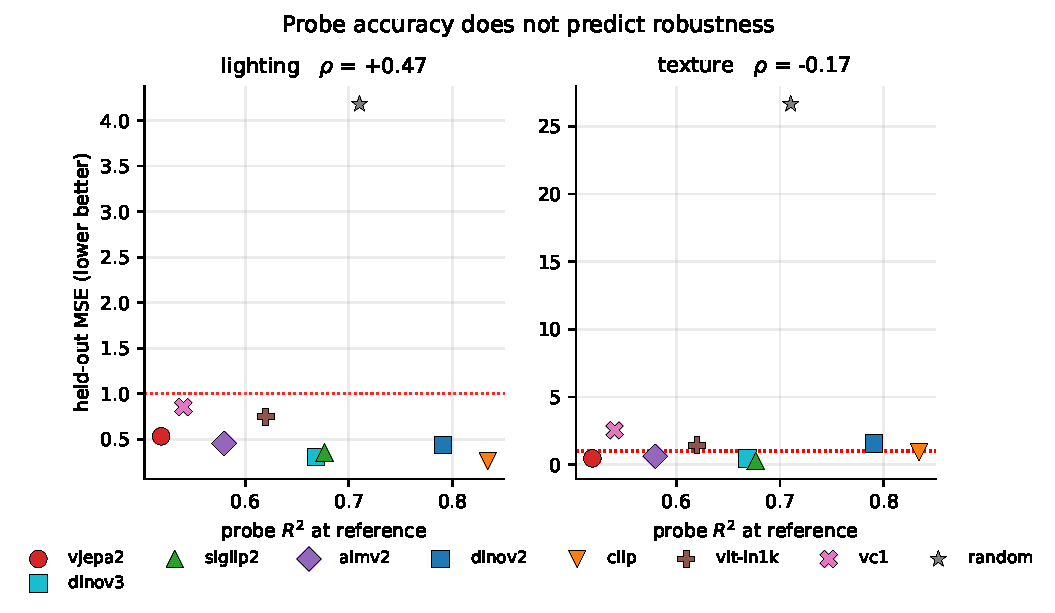
\includegraphics[width=\linewidth]{figures/fig1_probe_vs_robustness_push.pdf}
  \caption{\TODO{Caption should state the finding, not describe the axes.
  ``Probe accuracy at a shared reference condition (x) against held-out
  robustness (y). The relationship is absent and its sign varies by axis.''
  Note the red line at $1.0$ = no better than predicting the mean action.}}
  \label{fig:probe_vs_robustness}
\end{figure}

\begin{tabular}{l r r r r }
\toprule
encoder & probe $R^2$ & lighting & texture & clutter \\
\midrule
clip & 0.834 & 0.262 & 0.936 & 0.250 \\
dinov2 & 0.791 & 0.439 & 1.566 & 0.377 \\
random & 0.710 & 4.183 & 26.652 & 0.356 \\
siglip2 & 0.677 & 0.357 & 0.264 & 0.267 \\
dinov3 & 0.669 & 0.304 & 0.438 & 0.662 \\
vit-in1k & 0.620 & 0.747 & 1.433 & 0.538 \\
aimv2 & 0.580 & 0.456 & 0.607 & 0.400 \\
vc1 & 0.540 & 0.853 & 2.530 & 0.387 \\
vjepa2 & 0.519 & 0.533 & 0.462 & 0.381 \\
\midrule
Spearman $\rho$ & & +0.467 & -0.167 & excl. \\
\bottomrule
\end{tabular}

\TODO{Lead with the CLIP row --- best probe of all 15, first on lighting and
clutter, near-last on texture and viewpoint. That single row is the argument.}

\begin{figure}[t]
  \centering
  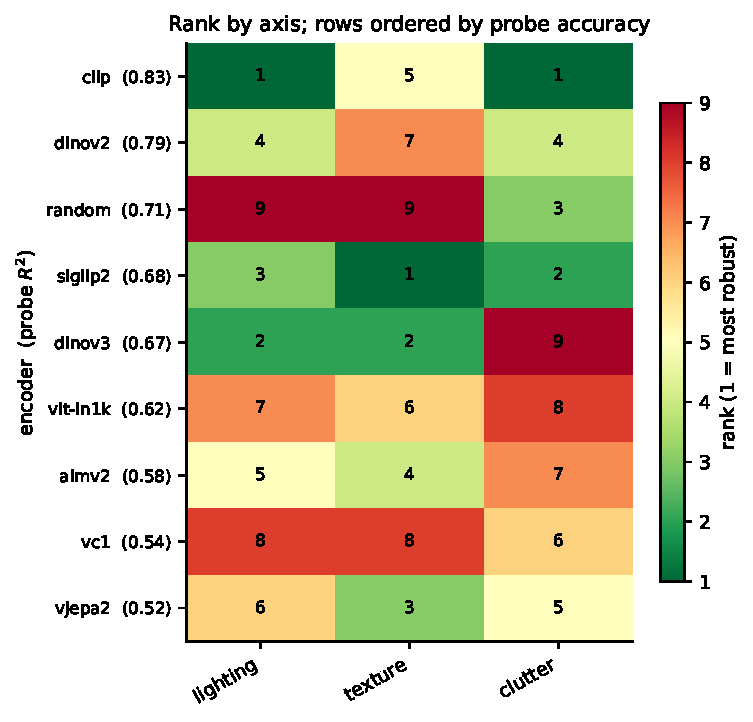
\includegraphics[width=0.8\linewidth]{figures/fig2_rank_heatmap_push.pdf}
  \caption{\TODO{Rank per axis, rows ordered by probe accuracy. A flat row
  would mean probe accuracy transfers; none is flat.}}
  \label{fig:rank_heatmap}
\end{figure}

\subsection{An axis that ranks nothing}
\TODO{Clutter. Frozen random features rank 3rd of 9, so the axis does not
discriminate and is excluded by a control registered in advance. Report it ---
a benchmark reporting distractor robustness on a task this insensitive reports
noise.}

\subsection{Latent distance against behaviour}
\begin{figure}[t]
  \centering
  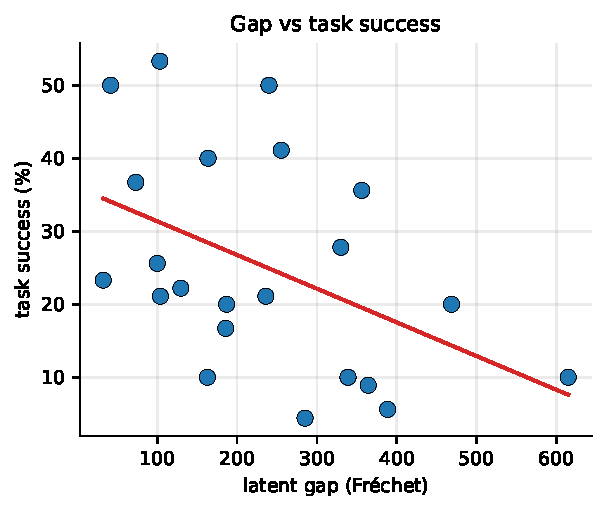
\includegraphics[width=0.55\linewidth]{figures/fig3_gap_vs_success.pdf}
  \caption{\TODO{$\rho = -0.52$ against task success, against $-0.85$ to
  $-0.92$ for world-model degradation on the same poses. The registered
  threshold was $-0.6$ and was missed; the interval excludes zero, so the
  relationship is real and weaker than assumed.}}
  \label{fig:gap_vs_success}
\end{figure}

\subsection{The floor nobody measures}
\begin{figure}[t]
  \centering
  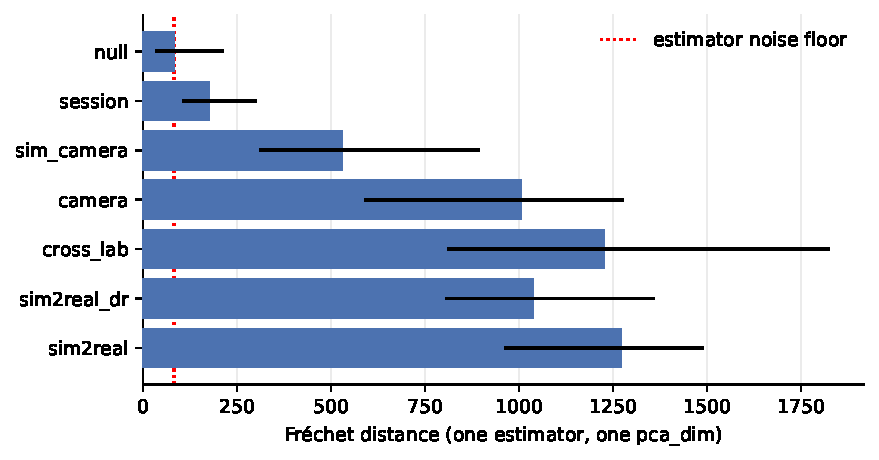
\includegraphics[width=0.8\linewidth]{figures/fig4_shift_ladder.pdf}
  \caption{\TODO{Session drift at $4.5\times$ the estimator's own noise floor,
  and a domain-randomised simulator sitting closer to a real laboratory than
  two real laboratories sit to each other.}}
  \label{fig:ladder}
\end{figure}

% ---------------------------------------------------------------------
\section{Limitations}
\label{sec:limitations}

\TODO{Write this section EARLY and honestly; it is the cheapest credibility in
the paper and reviewers punish omission far harder than admission.}

\begin{itemize}
  \item \TODO{Action MSE is not task success. \citet{criticalmse2026} argues it
        is a weak proxy. One leg is measured behaviourally ($\rho = -0.52$) and
        that is the stated size of the slack.}
  \item \TODO{No real robot. Every comparable claim in this literature was
        validated on hardware \citep{radosavovic2023mvp,burns2024what}.}
  \item \TODO{Two tasks; simulated nuisances; three seeds.}
  \item \TODO{Image-space axes are not physical simulations of their named
        phenomena.}
  \item \TODO{V-JEPA 2 sees two frames jointly; image encoders are averaged
        over pairs. Part of any video-encoder advantage is video-over-image.}
\end{itemize}

% ---------------------------------------------------------------------
\section{Conclusion}
\TODO{Three sentences. What was measured, what it means for practice, and the
one thing that would change it (hardware).}

\bibliographystyle{plainnat}
\bibliography{references}

\appendix
\section{Pre-registrations}
\TODO{The registrations were committed before each experiment ran, with
falsifiers named in advance, and several predictions failed. Point at the
repository. Do not oversell this --- one paragraph. Reviewers in this field are
largely indifferent to registration and framing it as a headline contribution
reads as substituting method for evidence.}

\section{Full results}
\TODO{Per-axis tables for both tasks, and the axes excluded by their controls.}

\end{document}
